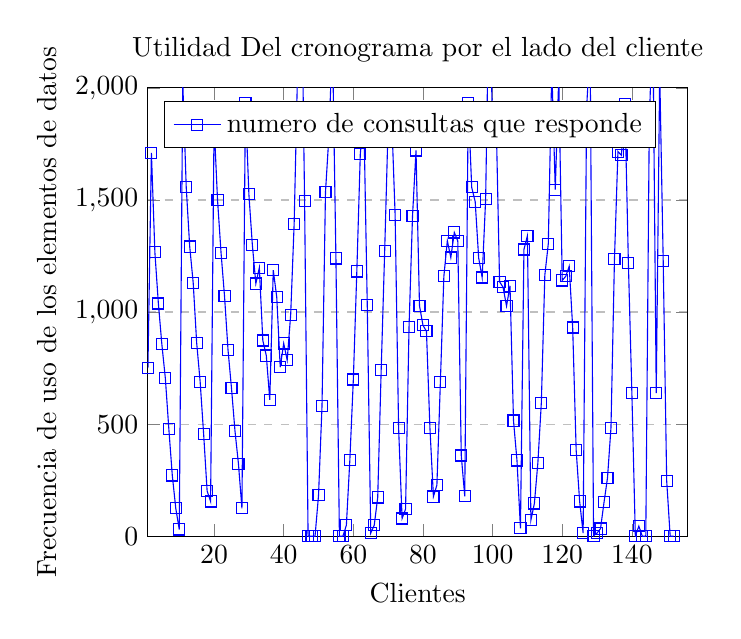
\begin{tikzpicture}
\begin{axis}[
    title={Utilidad Del cronograma por el lado del cliente},
    xlabel={Clientes},
    ylabel={Frecuencia de uso de los elementos de datos},
    xmin=1, xmax=156,
    ymin=0, ymax=2000,
    xtick={},
    ytick={},
    legend pos=north west,
    ymajorgrids=true,
    grid style=dashed,
]

\addplot[
    color=blue,
    mark=square,
    ]
    coordinates {
    %USO EXACTO
    (1,750)
(2,1710)
(3,1266)
(4,1038)
(5,856)
(6,705)
(7,480)
(8,271)
(9,124)
(10,30)
(11,2026)
(12,1557)
(13,1292)
(14,1131)
(15,863)
(16,689)
(17,456)
(18,202)
(19,155)
(20,1840)
(21,1498)
(22,1265)
(23,1071)
(24,832)
(25,661)
(26,470)
(27,323)
(28,124)
(29,1933)
(30,1525)
(31,1298)
(32,1127)
(33,1198)
(34,873)
(35,806)
(36,608)
(37,1187)
(38,1067)
(39,754)
(40,860)
(41,785)
(42,987)
(43,1394)
(44,2090)
(45,2646)
(46,1494)
(47,0)
(48,0)
(49,0)
(50,182)
(51,581)
(52,1535)
(53,1789)
(54,2218)
(55,1239)
(56,0)
(57,0)
(58,49)
(59,341)
(60,699)
(61,1181)
(62,1705)
(63,1881)
(64,1031)
(65,14)
(66,49)
(67,173)
(68,743)
(69,1271)
(70,1839)
(71,1873)
(72,1434)
(73,483)
(74,79)
(75,121)
(76,935)
(77,1429)
(78,1721)
(79,1028)
(80,941)
(81,914)
(82,482)
(83,177)
(84,228)
(85,688)
(86,1159)
(87,1318)
(88,1243)
(89,1355)
(90,1317)
(91,360)
(92,178)
(93,1934)
(94,1556)
(95,1492)
(96,1241)
(97,1154)
(98,1503)
(99,2484)
(100,1830)
(101,1880)
(102,1135)
(103,1111)
(104,1027)
(105,1117)
(106,516)
(107,338)
(108,35)
(109,1279)
(110,1340)
(111,72)
(112,146)
(113,327)
(114,596)
(115,1164)
(116,1305)
(117,2088)
(118,1546)
(119,2050)
(120,1141)
(121,1159)
(122,1204)
(123,931)
(124,384)
(125,155)
(126,14)
(127,1909)
(128,2195)
(129,2)
(130,14)
(131,34)
(132,151)
(133,260)
(134,484)
(135,1235)
(136,1716)
(137,1699)
(138,1928)
(139,1218)
(140,640)
(141,0)
(142,45)
(143,0)
(144,0)
(145,1836)
(146,2344)
(147,638)
(148,2069)
(149,1229)
(150,248)
(151,0)
(152,0)
    };
    \legend{numero de consultas que responde}

\end{axis}
\end{tikzpicture}

